
\section{Notizen, die ich später noch gebrauchen könnte}
............................................................

regelt horizontale Integration aus Produktionssicht und vertikale Integration des Assets aus IT-Sicht. Dabei werden die Daten über den gesamten Lebenszyklus von Prduktionsgegenständen/Komponenten gesammelt. Von typ zu Instanz.
Die Vertikale Sicht ist der Fokus dieser Arbeit.  Die vom Asset erzeugten Daten werden mit einer standardisierten Kommunikation (OPC UA) über den Kommunikationslayer an den funktional Player weitergegeben. Miaaaaau

Die senkrechte Achse bezieht sich auf die vertikale Integration des realen Produktionsgegenstandes (Asset), dessen virtuelle Repräsentation über die Integrantionsschicht erstellt wird. Zu den Assets werden sowohl alle in der Anlage verbauten physischen Komponenten als auch andere Vermögensgegenstände wie Software oder Patente, aber auch Menschen, gezählt \citep{Adolphs2017}.
 Über die Kommunikationsschicht

 Durch die horizontale Integration können technische, administrative sowie kommerzielle Daten über die gesamte Wertschöpfungskette hinweg konsisten gehalten werden.


Grundlage für neue Produkte zur Cloud-basierten Kommunikation


Die beiden horizontalen Achsen beschreiben Anforderungen und Voraussetzzungen für eine Industrie-4.0-Architektur aus Produktionssicht. In dieser Arbeit wird der Fokus auf die IT-Sicht gelegt. Daher wird die verikale Integration des Asstets genauer erläutert.
Auf vertikaler Achse wird das Asset, also der Gegenstand behandelt. Ziel ist die komplette Integration und die Vernezung der Produktionssysteme in Echtzeit. Asset-Layer, Integration-Layer, Commucation Layer-Standardisierte Kommunikation, Information Layer Datenhaltung, Functional



\begin{figure}[h]
  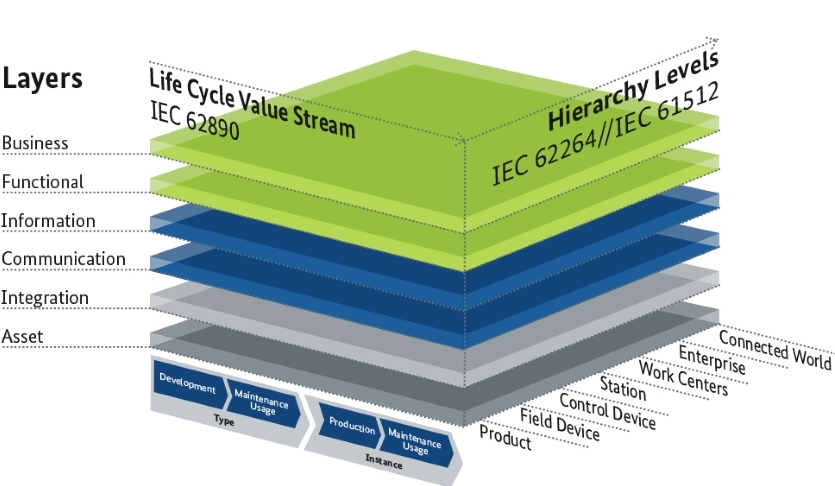
\includegraphics[width=1.0\linewidth]{RAMI.png}
  \caption[Das Referenzarchitekturmodell Industrie 4.0]{Das Referenzarchitekturmodell Industrie 4.0 \citep{BITKOM2015}}
  \label{fig:rami}
\end{figure}

\paragraph{Die Industrie-4.0-Komponente}


\begin{itemize}
  \item Bitkom bzw. Plattform Industrie 4.0 stellt Referenzarchitektur
  \item RAMI bietet die Möglichkeit, Industrie 4.0 UseCases zu verorten, um die für den jeweiligen use case notwendigen Normen und Standards zu identfizieren
  \item horizontale Integration über Wertschöpfungsnetzwerke: Lieferanten, Unternehmen, Produzenten
  \item Durchgängigkeit des Engineerings: Systems Engineering, Modellierung, Simulation
  \item vertikale Integration und vernetzte Pproduktionssysteme mit Echtzeitanforderung
  \item neue soziale Infrastrukturen der Arbeit: Humane-Machine-Systeme und Usability
  \item kontinuierliche Entwicklung von Querschnittssystemen: Netzkommunikation, Breitband, Cloud, Data Analytics, Cyber security
\end{itemize}

(Industrie 4.0 Weltweit)

Das RAMI 4.0 basiert auf den Grundideen des Smart Grids, welches das Stromnetz von der Erzeugung bis zur Verteilung zum Endverbraucher behandelt. Das dreidimensionale Modell kapselt die wichtigsten Funktionalitäten in mehreren Schichten. Dies schafft Flexibilität für die Konzeptionisierung und Realisierung von Industrie 4.0-Lösungen.

\begin{itemize}
  \item Aspekte Industrie 4.0 (Bitkom S. 40) -> Für diese Ziele muss eine Referenz geschaffen werden
  \item 1 - vertikale Integration innerhalb der Fabrik/der Produktion: Vernetzung von Produktionsmitteln wie Automatisierungsgeräte oder Dienste untereinander
  \item 2 - Einbeziehung der Produktes (in meinem Fall produzierte Energie)
  \item durchgängiges Engineering bedeutet: technische, administrative, kommerzielle Daten rund um das Produktionsmittel über Wertschöpfungskette hinweg konsistent halten und jederzeit über das Netzwerk zugreifbar machen
  \item 3 - horizontale Integration über Wertschöpfungsnetzwerke über den Fabrikstandort hinaus und dynamische Bildung von Wertschöpfungsnetzwerken
  \item es gibt RAMI 4.0
  \item und Referenzmodell für die Industrie 4.0-Komponente (s. 45) mit Verwaltungsschale
\end{itemize}


\begin{itemize}
  \item Disruption bestehender Geschäftsmodelle, vom Produzenten zum Dienstleister \citep{Doleski2017}
  \item dezentrale und fluktuierende Energieerzeugung erfordert digitale Lösungen
  \item wichtige Rolle kommunaler Unternehmen als Bereitsteller von Infrastrukturen wie Strom, Gas, Wärme, Wasser, Abwasser, Abfallwirtschaft, Stadtreinigung, Breitband \citep{Doleski2017}
  \item Beitrag zu funktionierendem Gemeinwesen, sozialer Teilhabe und Versorgungssicherheit -> Partner erster Wahl beim Gelingen der digitalen Transformation
  \item Wichtig für Gelingen: Erfahrungsaustausch, Kooperationen, richtige politische Rahmenbedingungen -> Katherine Reiche
  \item Trend: Energieversorgungsunternehmen wandeln sich Richtung Dienstleitsungsunternehmen
  \item politisch-regulatorisch auch angetrieben von ökologischen Zielen: In knapp 20 Jahren hat sich kein Sektor so radikal verändert wie der Energiesektor- Ende der 90er Jahre hat die Liberalisierung der Energiebranche die monopolitischen Strukturen der Versorgungsunternehmen  vertrieben. 2000 schon wurde das Erneuerbare-Energien-Gesetz verabschiedet uir systematischen Förderung regenerativer Energiequellen -> Energiewende(nach Fukushima 2011) zwang dann die Branchen sich strukturell in der Wertschöpfungskette zu verändern. Auch in Zukukunft wird die Branche sich rasant ändern! UND ANPASSUNGSFÄHIGKEIT IST A und O in DIGITALER QWELT
  \item gesellschaftlich: Stromanbieterwechsel ist sehr einfach geworden durch erhöhtes Angebot, daher müssen Anbieter sich stärker an Kundenwünschen orientieren. Kunden werden zum aktiven Teil der Wertschöpfung
\end{itemize}

\begin{enumerate}
  \item Ab 1998: Liberalisierung und Privatisierung der Strommärkte fördert Wettbewerb, stellt aber eine Herausforderung Digitalisierungsstrategie
  \item Ab 2011: Energiewende und Aussteig aus Kernenergie fördert neue Technologien für erneuerbare Energien, aber die Berechenbarkeit der Kapazitäten verändert sich
  \item Digitalisierung: Potenzial für neue Revolution, Strom kann zwar nicht digitalisiert werden, aber die Vertriebsmodelle
\end{enumerate}

Das Zusammenwachsen der pyhsischen und realen Welt zu mit Sensorik und Aktorik ausgestatteten Objekten, die mit dem Internet der Dinge miteinander vernetzt werden, erfordert eine Standardisierung \citep{BITKOM2015}.



Anforderung:Standardisierung


nach RAMI 4.0
RAMI (Referenzarchitekturmodell Industrie) 4.0: OPC-UA: Kommunikationsstandards (inkl. Sicherheit)
Sensorik: Bedeutung und sehr oberflächlich Funktionsweisen beschreiben
Gateways: Edge Processing
Device Management
Digital Twins
